%!TEX TS-program = pdflatex
\documentclass[ngerman]{article}

\usepackage[T1]{fontenc}
\usepackage{babel}
\usepackage{graphicx}
\usepackage{tikz}
\usepgflibrary{shapes.geometric}

\pagestyle{empty}
\usepackage[paperwidth=84.1cm, paperheight=118.9cm,margin=1cm]{geometry}

\begin{document}

\begin{center}
\begin{tikzpicture}
%\draw[step=1cm, blue, thin](0,0) grid (80,116);
%\draw[help lines,blue] (0,0) grid (80,115);
\node[anchor=north west ,inner sep=0] (frame1) at (3,113)     {\fbox{
\includegraphics[width=0.45\textwidth]{pg_0001}}};

\node[anchor=north west ,inner sep=0] (frame1) at (35,110)     {\fbox{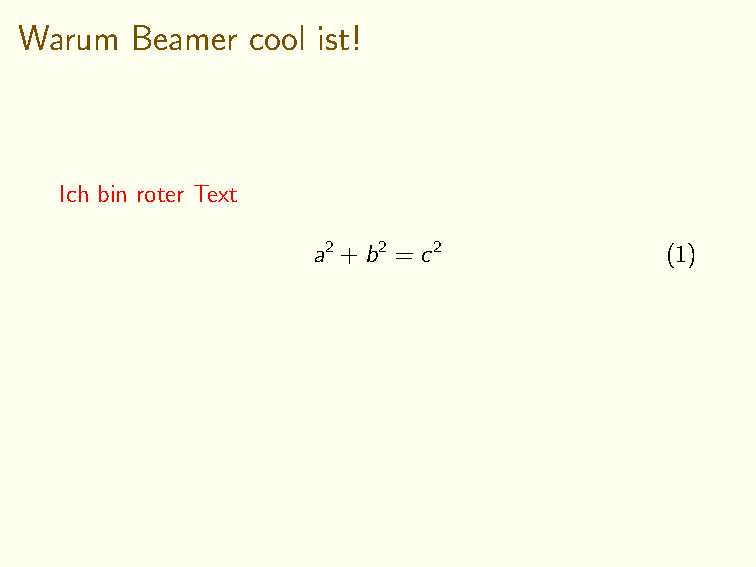
\includegraphics[width=0.45\textwidth]{pg_0003}}};

\node[anchor=north west ,inner sep=0] (frame1) at (5,80)     {\fbox{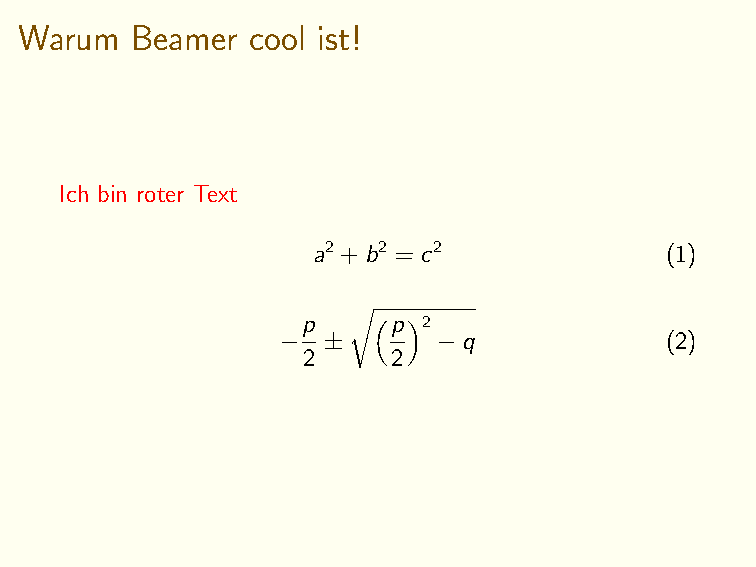
\includegraphics[width=0.45\textwidth]{pg_0004}}};

\node[anchor=north west ,inner sep=0] (frame1) at (35,75)     {\fbox{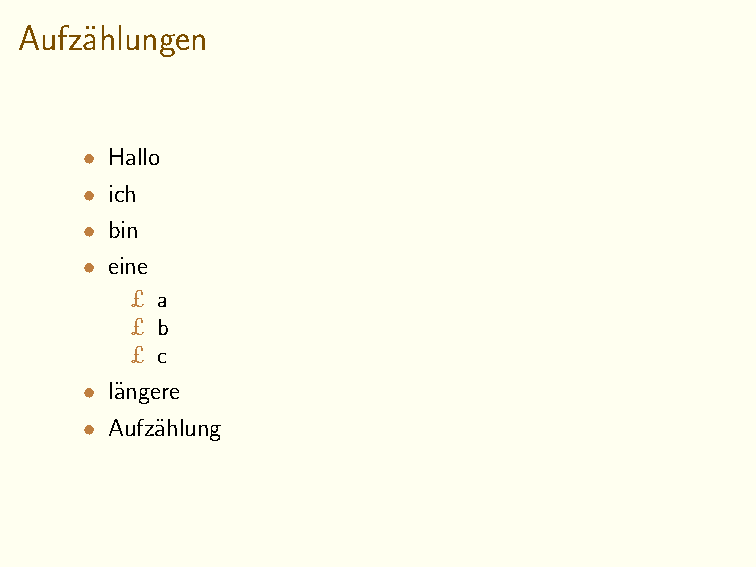
\includegraphics[width=0.45\textwidth]{pg_0005}}};

\node[anchor=north west ,inner sep=0] (frame1) at (5,45)     {\fbox{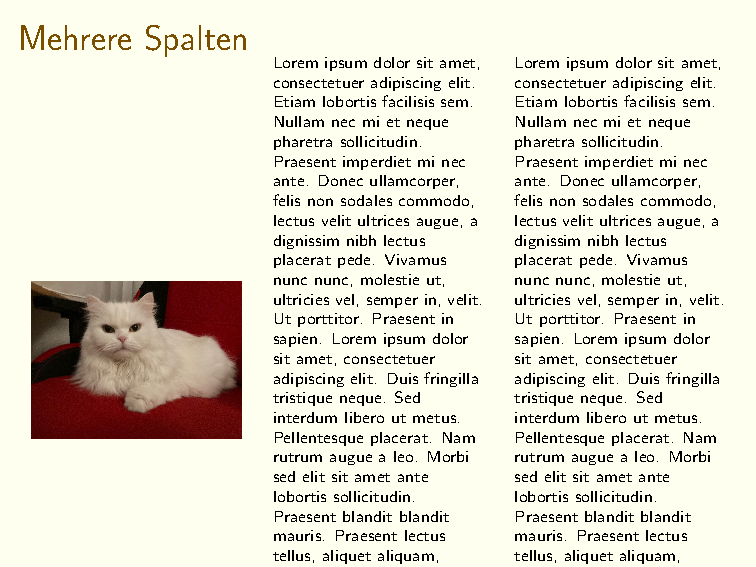
\includegraphics[width=0.45\textwidth]{pg_0006}}};

\node[anchor=north west ,inner sep=0] (frame1) at (41,35)     {\fbox{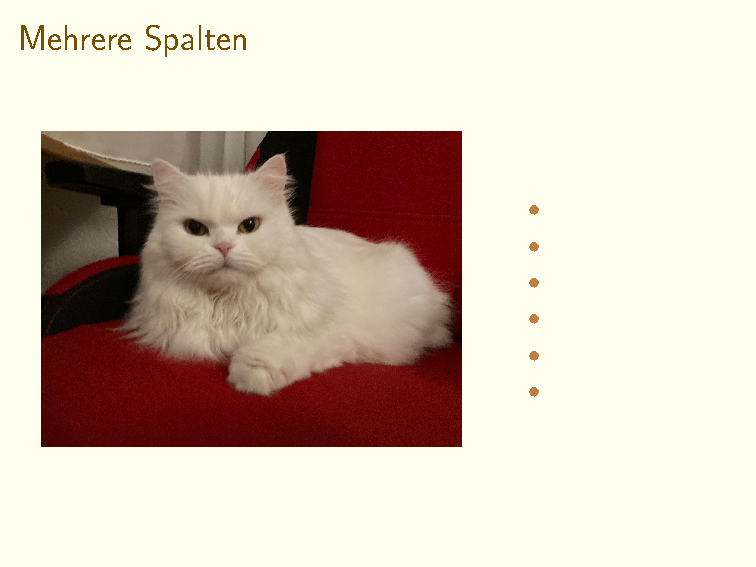
\includegraphics[width=0.45\textwidth]{pg_0007}}};


\node[anchor=north west ,inner sep=0] (frame2) at (10,10){\scalebox{10}{\bfseries stuff}};

\end{tikzpicture}
\end{center}

\end{document}